Una señal de sonido no es más que la variación en la presión que ejerce el medio que la transmite sobre su receptor.
La percepción del sonido en los seres humanos ocurre en dos regiones fundamentales: la \textit{periférica} y la \textit{nerviosa}.
Comienza en los oídos y continúa a través de la cóclea, en el oído interno, donde las variaciones en la presión del aire son transformadas en impulsos nerviosos conducidos hacia la corteza cerebral.

El hertz (Hz) es la unidad que expresa la cantidad de vibraciones que emite una fuente sonora en cada segundo de tiempo (frecuencia).
Se considera que el oído humano puede percibir ondas sonoras de frecuencias entre los 20 y los 20~000 Hz.
Los tonos agudos son percibidos en las frecuencias más altas (por encima de 5 kHz), y los graves en las bajas (menos de 250 Hz).

Un sonido puede ser representado de forma simple mediante un \textbf{oscilograma} (figura~\ref{img:oscillogram}), donde el eje X representa el tiempo, y el eje Y representa la \textit{amplitud} de la presión del sonido (generalmente usando unidades de media arbitrarias).
Mediante su análisis se pueden detectar con facilidad los instantes de tiempo de sonido más intensos y aquellos de silencio.

\begin{figure}[!h]
    \centering
    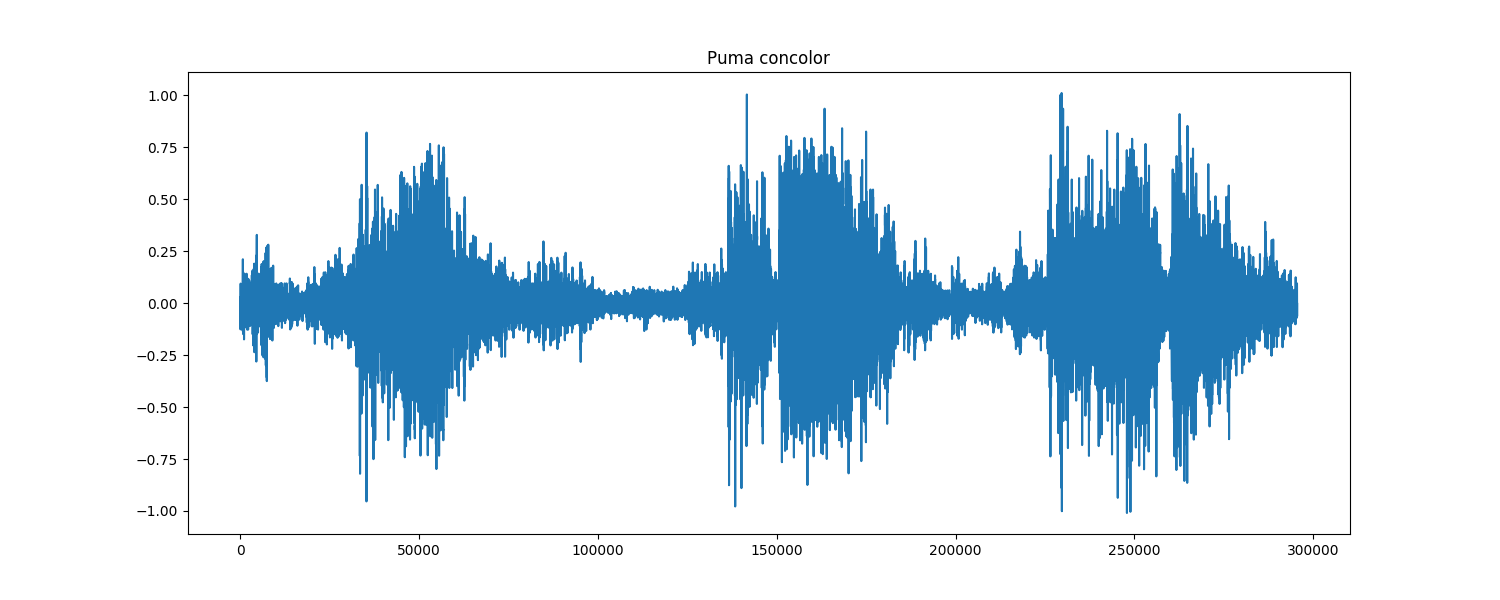
\includegraphics[width=\textwidth]{oscillogram.png}
    \caption{Oscilograma de una vocalización, de 2 segundos de duración, de un individuo de la especie \textit{ovis orientalis aries} (oveja doméstica).}
    \label{img:oscillogram}
\end{figure}

Una importante clase de sonidos son aquellos que consisten en oscilaciones que se repiten periódicamente cada un cierto tiempo.
La duración de una de estas oscilaciones es conocida como su \textit{período} (en segundos) y a la medida inversa se le denomina \textit{frecuencia} (en Hz).
Otro grupo de señales sonoras, llamadas \textit{armónicas} es igualmente interesante, pues se trata de señales compuestas por varias oscilaciones periódicas cuyas frecuencias son todas múltiplos de la más baja presente en la señal.
Existen, asimismo, otros sonidos de características aleatorias y que no se repiten periódicamente, llamados \textit{ruidos}.

Una oscilación puede ser descompuesta en una suma de sinusoides elementales de diferentes frecuencias, mediante la aplicación de la \textbf{transformada de Fourier}.
La representación de la transformada de Fourier de una señal en un tiempo dado es conocida como su \textbf{espectro} (figura~\ref{img:spectrum+spectrogram}a).
Esta transformada puede ser igualmente computada sobre pequeñas tramas de tiempo superpuestas, lo que produce una representación tridimensional de la intensidad de las frecuencias en el tiempo, que llamamos \textbf{espectrograma} (figura~\ref{img:spectrum+spectrogram}b).

\begin{figure}[!h]
    \centering
    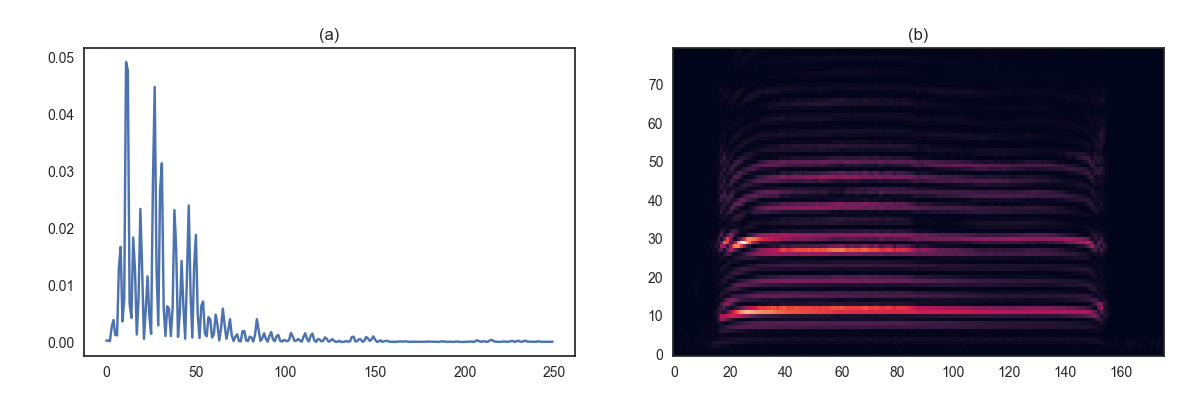
\includegraphics[width=\textwidth]{spectrum+spectrogram.png}
    \caption{Representaciones de la transformada de Fourier de la señal de la figura~\ref{img:oscillogram}: (a) Espectro de una trama. (b) Espectrograma.}
    \label{img:spectrum+spectrogram}
\end{figure}

Para el procesamiento computacional de una señal, esta debe ser llevada del dominio analógico al digital, para lo cual se discretiza mediante observaciones realizadas a intervalos regulares.
Los pasos más importantes en esta conversión de la señal de analógica a digital son:

\begin{enumerate}
    \item \textbf{Filtrado}: La señal analógica se filtra con el propósito de limitar las frecuencias presentes al intervalo $[0,B]$, donde $B$ es la frecuencia \textit{máxima} o \textit{de corte}.
    \item \textbf{Muestreo}: Se digitaliza la señal resultante del paso anterior;
    se emplea \textit{frecuencia de muestreo} $F_s = 2B$ para evita el fenómeno de \textit{aliasing}\footnote{Efecto que causa que señales continuas distintas se tornen indistinguibles cuando se muestrean digitalmente si la tasa de muestreo es menor que el doble de la frecuencia más alta.
    Cuando esto sucede, la señal original no puede ser reconstruida de forma unívoca a partir de la señal digital.}.
    \item \textbf{Cuantificación}: La señal digital es cuantificada, se limita el espacio de almacenamiento ocupado por cada muestra.
\end{enumerate}

Para una calidad de audio de CD se emplean valores de muestreo $F_s = 44.1$ kHz y una cuantificación de 16 bits por muestra.

Los algoritmos de inteligencia artificial tradicionalmente operan con vectores numéricos, llamados \textit{vectores de características}.
En las siguientes secciones analizamos los procedimientos mediante los cuales una señal de audio digital se transforma en una secuencia de tales vectores.

Al procesar una grabación sonora, determinados intervalos de tiempo y/o frecuencias pueden resultar más <<importantes>> que otros.
Estas secciones, conocidas como \textit{segmentos}, permiten establecer una correspondencia entre un evento de sonido y un individuo de una especie dada.
La segmentación, por lo tanto, simplifica la tarea de clasificar una señal acústica;
y las operaciones de procesamiento y extracción de características que se mencionan en lo adelante se aplican sobre dichos segmentos.

\section{Tramas}\label{sec:frames}
Para procesar una señal esta a menudo es dividida en pequeños segmentos, conocidos como \textit{tramas}\footnote{\textit{frames} en inglés.}, de longitud constante y espaciados en intervalos de tiempo iguales.
Denotamos por $N$ la cantidad de muestras de la señal que contiene una trama;
de esta forma la duración de una trama será de $N/F_s$.
Asimismo, denotamos por $M$ la cantidad de muestras en que difieren dos tramas consecutivas, conocida como \textit{tamaño de paso}, y que usualmente es menor que $N$.
A partir de estos valores podemos igualmente calcular la cantidad de muestras que dos tramas consecutivas tienen en común, como $N-M$;
y el número de tramas por segundo (\textit{frame rate}) como $F_s/M$.

Cada trama de $N$ muestras es usualmente obtenida mediante la aplicación de una función \textit{ventana} $w(n)$ a la señal, que es distinta de cero solo si $0\leq n\leq N-1$.
Dada la señal $s[n]$, una trama que comienza en la muestra $m$ es obtenida como

\begin{equation}
    \label{eq:windowing}
    s[n]_m = \begin{cases}
                 s[n + m]w(n) & 0\leq n\leq N-1 \\
                 0 & eoc.
    \end{cases}
\end{equation}

% TODO Move this to a table
Dos de las variantes más conocidas para la función $w(n)$ son las siguientes:

\begin{itemize}
    \item \textbf{Rectangular}:
    \begin{equation*}
        w(n) = \begin{cases}
                   1 & 0\leq n\leq N-1 \\
                   0 & eoc.
        \end{cases}
    \end{equation*}
    \item \textbf{Hamming}:
    \begin{equation*}
        w(n) = 0.53836 - 0.46164 \cos\left(\frac{2\pi n}{N-1}\right)
    \end{equation*}
\end{itemize}

La elección de la ventana $w(n)$ tiene un efecto sobre los resultados de operaciones posteriores sobre las tramas obtenidas.
En la práctica, algunos métodos de procesamiento, como la transformada de Fourier producen mejores resultados cuando se emplean funciones que se aproximan a cero en sus extremos, como la de Hamming.

Una vez computados, los valores asociados a una característica de la señal para cada trama suelen ser <<generalizados>> para representar su comportamiento global.
El procedimiento varía desde la generación de nuevas características a partir de las ya calculadas~\cite{Giret11}, hasta la simplificación de estas a la media y varianza de cada una de sus componentes.
Esto es especialmente importante para el empleo de dichos vectores en algoritmos de inteligencia artificial, puesto que las señales no siempre se descomponen en un mismo número de tramas;
mientras que aplicando este método, el tamaño de los vectores de características sí será igual para todas, lo cual es un requisito de muchos de dichos algoritmos.

\section{Características temporales}\label{sec:característicasTemporales}
Las características temporales, que describen las propiedades de la señal en el dominio del tiempo, son muy simples;
y se computan directamente a partir de la señal digitalizada.
A continuación se mencionan varias de ellas.

\subsection{Log-Attack Time}\label{subsec:log-attackTime}

El \textit{attack} de una señal se define como el espacio de tiempo, al inicio de esta, en que su intensidad va en ascenso.

El \textit{log-attack time} (LAT)~\cite{Gunasekaran11,Kim05,Manjunath02,Peters04} se calcula entonces como el logaritmo en base 10 de la duración del intervalo de tiempo transcurrido entre los momentos en que la señal se hace audible ($startAttack$) y en que alcanza su máxima intensidad ($stopAttack$):

\begin{equation}
    \label{eq:LAT}
    LAT = \log_{10}{(stopAttack - startAttack)}
\end{equation}

Específicamente, los momentos $stopAttack$ y $startAttack$ suelen definirse como los puntos en que la potencia de la señal alcanza el 20\% y el 90\% de su máximo respectivamente.

\subsection{Audio Waveform}\label{subsec:audioWaveform}

Para computar esta característica se divide la señal en tramas no superpuestas ($M = N$), y se computan, por cada trama, los 2 valores siguientes:

\begin{itemize}
    \item Menor valor de amplitud de la señal presente en la trama.
    \item Mayor valor de amplitud de la señal presente en la trama.
\end{itemize}

El \textit{audio waveform} (AWF)~\cite{Kim05,Manjunath02} de la señal consistirá en un vector con los pares calculados, correspondientes a cada una de dichas tramas.

La extracción del AWF puede ser vista como un modo de <<compresión>> de la señal.
Si se toma $N=1$ se obtendrá la propia señal, mientras que a medida que se seleccionen valores de $N$ más altos, el número de valores resultantes será cada vez menor, obteniéndose una representación reducida de la señal original.
El AWF puede representarse gráficamente como un conjunto de segmentos con extremos en los valores de la tupla correspondiente y ubicados según el momento en que ocurren en la señal (figura~\ref{img:awf+ap}).

\subsection{Audio Power}\label{subsec:audioPower}

El \textit{audio power} (AP)~\cite{Kim05,Manjunath02} describe el comportamiento de la potencia de la señal en cada instante de tiempo.
Al igual que para la AWF, su cálculo requiere dividir la señal en tramas no superpuestas;
y se computa, para la trama $x[n]$ mediante la siguiente expresión:

\begin{equation}
    \label{eq:AP}
    AP = \frac{1}{N}\sum_{n=0}^{N-1}{|x[n]|^2}
\end{equation}

La representación gráfica del AP posibilita el análisis directo de la evolución de la amplitud de la señal en el transcurso del tiempo, lo que puede observarse en la figura~\ref{img:awf+ap}.

\begin{figure}[!h]
    \centering
    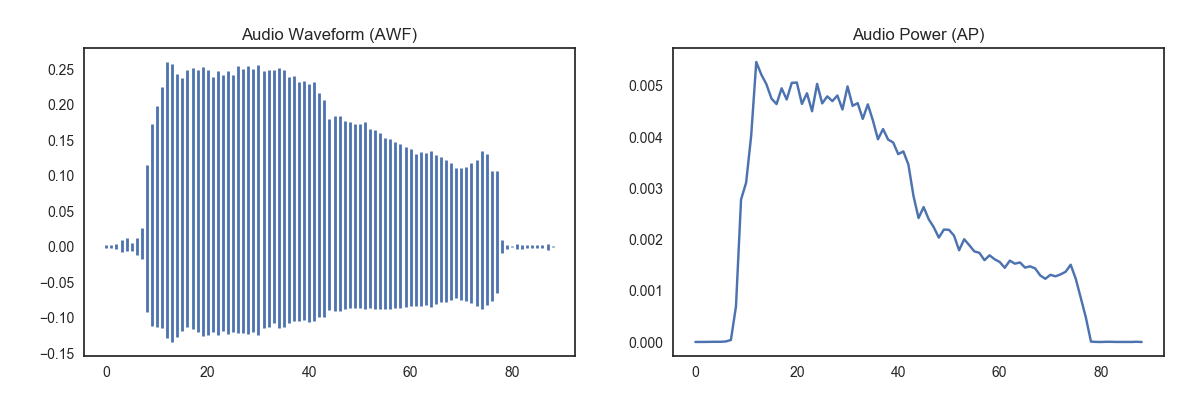
\includegraphics[width=\textwidth]{temporal-features.png}
    \caption{Dos características temporales básicas de una señal de audio: \textit{Audio Waveform} y \textit{Audio Power}, correspondientes a la señal de la figura~\ref{img:oscillogram}.}
    \label{img:awf+ap}
\end{figure}

\subsection{Temporal Centroid}\label{subsec:temporalCentroid}

El \textit{temporal centroid} (TC)~\cite{Kim05,Manjunath02,Peters04,Zamanian17} de la señal es el punto donde se localiza el centro de masas de su AP\@.
Se calcula mediante la siguiente expresión:

\begin{equation}
    \label{eq:TC}
    TC = \frac{\sum_{t=0}^{T-1}{AP_t \cdot t}}{\sum_{t=0}^{T-1}{AP_t}}
\end{equation}

\noindent
donde $T$ es la cantidad de tramas en que se descompuso la señal.

\subsection{Effective Duration}\label{subsec:effectiveDuration}

La \textit{effective duration} (ED)~\cite{Peters04} de una señal constituye la duración del intervalo de tiempo en que esta es perceptible;
el que generalmente se considera como el intervalo en que la amplitud de la señal permanece por encima del 40\% de su valor máximo.

\subsection{Auto-correlation}\label{subsec:auto-correlation}

La \textit{auto-correlation} (AC)~\cite{Gunasekaran11,Peters04} de la señal está dada por un vector de coeficientes que describen su distribución espectral en el dominio del tiempo.
El coeficiente $k$-ésimo se calcula mediante la expresión:

\begin{equation}
    \label{eq:AC}
    AC_k = \frac{1}{x[0]^2}\sum_{n=0}^{N-k-1}{x[n]\cdot x[n+k]}
\end{equation}

\subsection{Zero Crossing Rate}\label{subsec:zeroCrossingRate}

El \textit{zero crossing rate} (ZCR)~\cite{Fagerlund07,Gunasekaran11,Peters04} es una medida del número de veces que la amplitud de la señal cambia de signo.
Los sonidos periódicos tienden a tener un pequeño valor de ZCR, mientras que para los ruidos este valor suele ser alto.

Puede ser computado de forma global, o para cada trama de la señal, aplicando la siguiente expresión:

\begin{equation}
    \label{eq:ZCR}
    ZCR = \frac{1}{2}\sum_{n=1}^{N-1}{|\text{sign}(x[n]) - \text{sign}(x[n-1])|}
\end{equation}


\section{Características espectrales}\label{sec:característicasEspectrales}
Las características de esta categoría describen la representación de las señales de sonido en el dominio de las frecuencias.

Una trama $x[n]$, de longitud $N$, tiene una representación en el dominio de las frecuencias que puede ser obtenida mediante la aplicación de la \textbf{transformada discreta de Fourier} (DFT por sus siglas en inglés):

\begin{equation}
    \label{eq:DFT}
    X[f] = \sum_{n=0}^{N-1}{x[n]e^{\frac{-i2\pi fn}{N}}}
\end{equation}

El espectro $X[f]$ puede ser transformado de vuelta al dominio del tiempo aplicando la \textbf{transformada discreta inversa de Fourier} (IDFT):

\begin{equation}
    \label{eq:IDFT}
    x[n] = \frac{1}{N}\sum_{f=0}^{N-1}{X[f]e^{\frac{i2\pi fn}{N}}}
\end{equation}

Al ser $x[n]$ un vector de valores reales, podemos aplicar sobre este una propiedad de la DFT que plantea que el vector $X[f]$ es, por tanto, conjugado simétrico, por lo que suelen considerarse solamente los últimos $\lceil (N+1)/2 \rceil$ valores de este.

La posición $k$-ésima del vector $X[k]$ contiene la amplitud correspondiente a la frecuencia $k(F_s/N)$ en la señal.

Podemos definir $X[f,t]$ como la matriz compuesta por las DFTs correspondientes a cada una de las tramas de una señal, donde el valor en la posición $(f, t)$ corresponde a la amplitud de la frecuencia $f$ en la trama $t$.
A partir de esta matriz se construye el espectrograma de la señal.

\subsubsection{Spectral Centroid}

El \textit{spectral centroid} (SC) constituye el centro de masas del espectro de frecuencias de una trama, y permite describir la señal en términos del tipo de frecuencias predominantes (altas o bajas) en cada trama.
Puede computarse mediante la siguiente expresión:

\begin{equation}
    \label{eq:SC}
    SC = \frac{\sum_{k=0}^{K-1}{f(k)|X[k]|}}{\sum_{k=0}^{K-1}{|X[k]|}}
\end{equation}

\noindent
donde $K$ es la longitud del vector correspondiente a la DFT de la trama, y $f(k)$ frecuencia asociada a la posición $k$-ésima de este.

\subsubsection{Spectral Spread}

También conocido como \textit{instantaneous bandwith} o \textit{spectral width}, el \textit{spectral spread} (SS) de una señal refleja la dispersión del espectro de frecuencias en torno a su centroide.

Puede calcularse aplicando la siguiente expresión en cada trama:

\begin{equation}
    \label{eq:SS}
    SS = \sqrt{\frac{\sum_{k=0}^{K-1}{\left[ \log_{2}{(f(k))-SC} \right]^2 |X[k]|}}{\sum_{k=0}^{K-1}{|X[k]|}}}
\end{equation}

\noindent
donde $X[k]$ es la DFT de la trama, y tiene cardinalidad $K$.

Valores bajos (característicos de sonidos armónicos) del SS expresan una concentración de las amplitudes alrededor de la frecuencia centroide;
los valores altos (propios de ruidos), en cambio, muestran una dispersión de las amplitudes en un rango de frecuencias mayor.

\subsubsection{Spectral Roll-off}

El \textit{spectral roll-off} (SRO) se define como la frecuencia bajo la cual se encuentra un porcentaje específico (usualmente entre el 85\% y el 99\%) de la energía espectral total.

\subsubsection{Spectral Flux}

Caracteriza la variación dinámica de la información espectral.
El \textit{spectral flux} (SFX) se calcula como la norma de la diferencia entre los espectros de dos tramas consecutivas.
El coeficiente correspondiente a la trama $t$, $t\geq 1$, puede calcularse entonces aplicando:

\begin{equation}
    \label{eq:SFX}
    SFX_t = ||\hat{X}_t -\hat{X}_{t-1}||
\end{equation}

\noindent
donde $\hat{X}_t$ es la transformada discreta de Fourier de la trama $t$-ésima de la señal.

\subsubsection{Spectral Flatness}

El \textit{spectral flatness} (SF) de una señal refleja su similitud a una señal compuesta por ruido, caso en que su valor se aproxima a 1;
mientras que si se trata de una señal armónica, el valor será próximo a 0.

El SF se calcula como la razón entre las medias geométrica y aritmética de las amplitudes presentes en la DFT de la trama, es decir, mediante la expresión:

\begin{equation}
    \label{eq:SF}
    SF = \frac{\prod_{k=0}^{K-1}{|X[k]|}^{\frac{1}{K}}}{\frac{1}{K}\sum_{k=0}^{K-1}{|X[k]|}}
\end{equation}

\noindent
donde $X[k]$ es la DFT de la trama, de cardinalidad $K$.

\begin{figure}[!h]
    \centering
    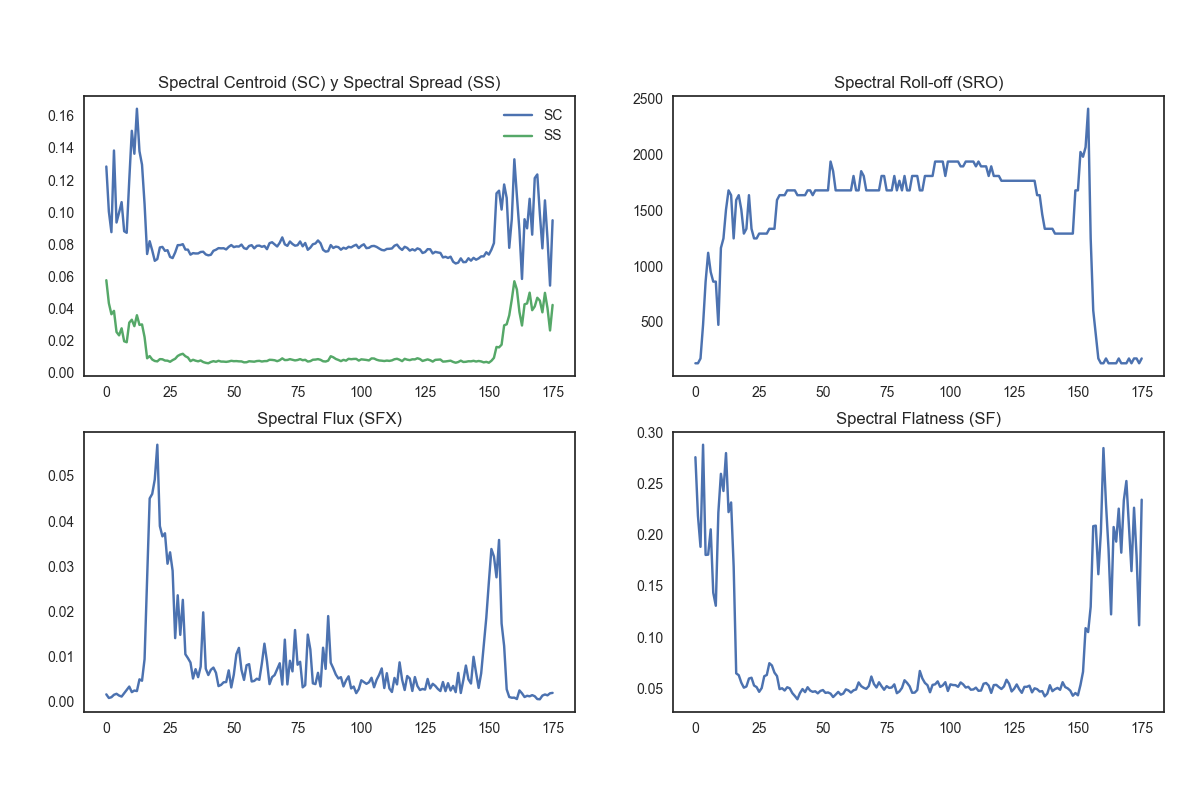
\includegraphics[width=0.95\textwidth]{spectral-features.png}
    \caption{Características espectrales básicas de una señal de audio.}
    \label{img:basic-spectral-descriptors}
\end{figure}

\section{Características armónicas}\label{sec:característicasArmónicas}
Las características incluidas en este grupo describen el grado de armonicidad de la señal, o sea, su composición en términos de señales puramente armónicas.

La extracción de estos descriptores requiere la estimación de la \textbf{frecuencia fundamental} de la señal, así como de los llamados \textbf{picos armónicos}.

La frecuencia fundamental ($F_0$) es la frecuencia más baja del espectro de frecuencias tal que las frecuencias dominantes en la señal pueden expresarse como múltiplos de ella.
Puede entonces considerarse la $F_0$ como la frecuencia de la señal armónica que mejor representa a la señal en cuestión.

Existen numerosas variantes para la estimación de la $F_0$ de una señal~\cite{Kim05}, siendo la propuesta en~\cite{Cheveigne02} una de las más empleadas.
Esta técnica, también conocida como \textit{algoritmo YIN}, se basa a grandes rasgos en encontrar el valor del período $\tau$ que minimiza la función $d_t'(\tau)$ para cada trama $t$~\cite{Gerhard03-2}:

\begin{gather}
    \label{eq:YIN}
    d_t'(\tau) = \begin{cases}
                     1 & \tau = 0 \\
                     \frac{d_t(\tau)}{\frac{1}{\tau}{\sum_{j=1}^{\tau}{d_t(j)}}} & eoc.
    \end{cases}\\
    d_t(\tau) = \sum_{i=0}^{N-1}{(x[i]-x[i+\tau])^2}
\end{gather}

Luego, la frecuencia fundamental estará dada por la expresión $F_0 = 1/\tau$.

Conocida la frecuencia fundamental de la señal, pueden estimarse sus picos armónicos, los que se localizan en torno a los múltiplos de $F_0$.
De esta forma, se puede definir el $h$-ésimo pico armónico como el valor de la DFT de la señal localizado en la posición $k_h$ tal que:

\begin{equation}
    \label{eq:harmonicPeaks}
    k_h = \argmax_{k\in [a_h,b_h]}|X[k]|
\end{equation}

\noindent
donde los extremos del intervalo $[a_h, b_h]$ están dados por las ecuaciones:

\begin{gather*}
    a_h = \text{floor}\left[ (h - nht)\frac{F_0}{\Delta F} \right] \\
    b_h = \text{ceil}\left[ (h + nht)\frac{F_0}{\Delta F} \right]
\end{gather*}

\noindent
y donde $\Delta F = F_{s}/K$ es el intervalo de frecuencias entre dos posiciones consecutivas de la DFT de la señal, $K$ es cardinalidad de la DFT\@.
$nht$ es un valor denominado \textit{tolerancia no armónica}, usualmente tomado como $nht = 0.15$.

El procedimiento presentado para la estimación de los picos armónicos no siempre produce buenos resultados si las características de la señal difieren en extremo de las de una señal armónica.
Otras variantes más apropiadas para tales casos han sido diseñadas, basadas en la descomposición del proceso en dos pasos: primero la detección de \textit{picos espectrales} y luego los picos armónicos.
En esencia, se detectan todos los picos presentes en la DFT de la señal y luego se comparan con los de la señal armónica correspondiente a la frecuencia fundamental.
Al final, se conservan los picos que mejor se ajusten a los de la señal armónica~\cite{Kim05}.

\subsection{Inharmonicity}\label{subsec:inharmonicity}

La \textit{inharmonicity} (INH)~\cite{Peters04,Zamanian17} representa la divergencia de las frecuencias que componen la señal respecto a los múltiplos de su frecuencia fundamental.
Se calcula mediante la expresión:

\begin{equation}
    \label{eq:INH}
    INH = \frac{2}{F_0} \cdot \frac{\sum_{h}{|f(h) - h\cdot F_0|\cdot |X[h]|^2}}{\sum_{h}{|X[h]|^2}}
\end{equation}

\noindent
donde $h$ itera por los picos armónicos de la señal, y $f(h)$ y $X[h]$ son respectivamente la frecuencia asociada al pico $h$-ésimo y el valor del coeficiente correspondiente de la DFT\@.

Los valores de la INH varían entre 0 (señal puramente armónica) y 1 (señal no armónica).

\subsection{Odd to Even Harmonic Energy Ratio}\label{subsec:oddToEvenHarmonicEnergyRatio}

Este descriptor~\cite{Gunasekaran11,Peters04} permite distinguir entre sonidos donde predominan los múltiplos pares de la frecuencia fundamental, de aquellos donde predominan los impares, o donde ambos tienen amplitudes equivalentes.
Se computa como el cociente entre las posiciones de la DFT de la señal correspondientes a picos armónicos impares y las correspondientes a picos pares:

\begin{equation}
    OER = \frac{\sum_{h=2p+1}{|X[h]|^2}}{\sum_{h=2p}{|X[h]|^2}}, p\in\mathbb{N}\cup \{ 0 \}
\end{equation}

\subsection{Tristimulus}\label{subsec:tristimulus}

El \textit{tristimulus} (TR)~\cite{Gunasekaran11,Peters04} fue introducido como un equivalente a los atributos de color en la visión.
Se calcula para tres conjuntos de picos armónicos, agrupados de forma equivalente al modo en que son percibidos en la audición humana.
Las fórmulas para los tres coeficientes son las siguientes:

% TODO Check this way of calling peaks with lower indices
\begin{equation}
    \begin{aligned}
        T1 & = \frac{|X[h_0]|}{\sum_{h}{|X[h]|}} \\
        T2 & = \frac{|X[h_1]|+|X[h_2]|+|X[h_3]|}{\sum_{h}{|X[h]|}} \\
        T3 & = \frac{\sum_{h\in \{h_4, h_5, \ldots, h_{H-1}\}}{|X[h]|}}{\sum_{h}{|X[h]|}}
    \end{aligned}
\end{equation}

\noindent
donde $H$ es la cantidad total de picos armónicos en la señal, y $h_i$ el pico $i$-ésimo.
El denominador es, en los tres casos, la suma de las amplitudes de las frecuencias de todos los picos armónicos.

Como se puede observar, el primer coeficiente corresponde solamente a la proporción de la energía contenida en el primer pico, $T2$ a los picos del segundo al cuarto, y $T3$ a los restantes.

\begin{figure}[!h]
    \centering
    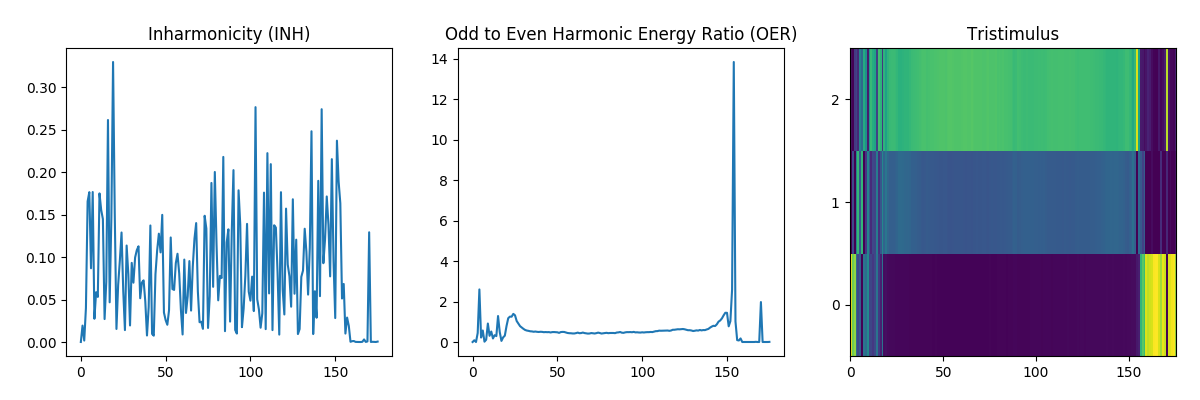
\includegraphics[width=\textwidth]{harmonic-features.png}
    \caption{Características armónicas básicas correspondientes a la señal representada en la figura~\ref{img:oscillogram}.}
    \label{img:harmonic-features}
\end{figure}


\section{Mel Frequency Cepstral Coefficients}\label{sec:MFCC}
Los \textit{Mel Frequency Cepstral Coefficients} (MFCC)~\cite{Davis80} son coeficientes para la representación del habla basados en la percepción auditiva humana.
Su objetivo es caracterizar el contenido relevante de la señal, obviando aquellas características que poseen información poco valiosa como el ruido de fondo, emociones, volumen, tono, etc.
Si bien fueron desarrollados para tareas asociadas al reconocimiento automático del habla, igualmente han tenido una amplia aplicación en áreas relacionadas al procesamiento de señales musicales y bioacústicas~\cite{McKinney03,Dufour14,Clemins05,Lee06,Li01,Cowling03,Mitrovic06,Fagerlund07}.

Los MFCC se basan en la característica del sistema auditivo humano que provoca que para este sea más difícil discernir entre dos frecuencias cercanas cuanto más altas ellas sean.
La \textbf{escala Mel} (figura~\ref{img:mel-scale}) fue desarrollada con el propósito de representar esta propiedad, permitiendo medir las frecuencias de un modo más acorde a la percepción humana de estas, mediante el uso de la unidad de medida conocida como \textit{Mel}.

\begin{figure}[!h]
    \centering
    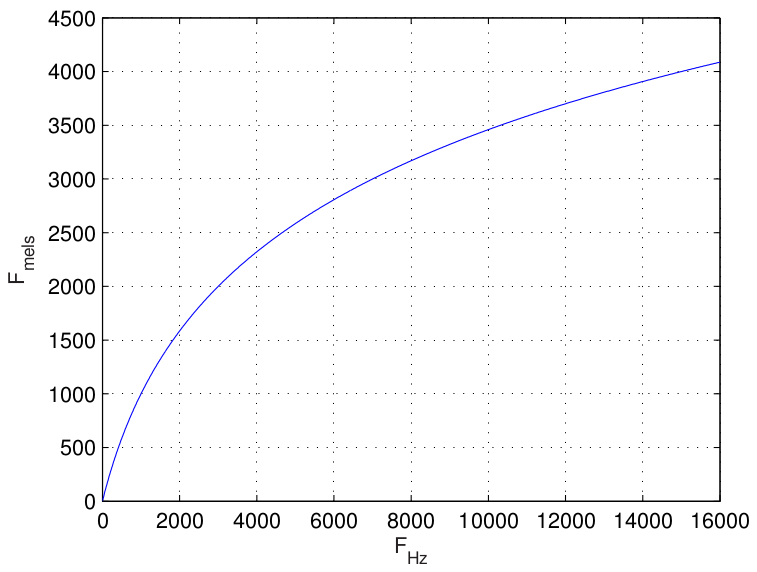
\includegraphics[width=0.5\textwidth]{mel-scale.png}
    \caption{Correspondencia entre las unidades de medida de frecuencias \textit{Hz} y \textit{Mel} de acuerdo con la escala Mel.}
    \label{img:mel-scale}
\end{figure}

La conversión de Hertz ($f$) a Mel ($m$) se realiza aplicando la ecuación~(\ref{eq:Hz-Mel}), mientras que por~(\ref{eq:Mel-Hz}) se puede convertir en sentido contrario.

\begin{equation}
    \label{eq:Hz-Mel}
    m = 2595\log_{10}\left( 1 + \frac{f}{700} \right)
\end{equation}

\begin{equation}
    \label{eq:Mel-Hz}
    f = 700\left( 10^{m/2595} - 1 \right)
\end{equation}

Una ventaja de la escala Mel es que nos permite definir los llamados \textbf{bancos de filtros de Mel}, mediante los cuales podemos <<resumir>> la energía de una señal en $M$ regiones de frecuencias repartidas en correspondencia con la escala Mel (más distanciadas a medida que las frecuencias se hacen mayores).
Para ello, dividimos el intervalo de frecuencias presente en la señal en $M+2$ puntos igualmente distanciados.
A continuación los convertimos a Mel, de forma que ahora estos estarán situados a distancias correspondientes a la percepción humana de las frecuencias.
Luego, definimos los $M$ filtros mediante la siguiente fórmula:

\begin{equation}
    \label{eq:Mel filterbank}
    H_m(k) = \begin{cases}
                 0 & k < f_{m-1} \\
                 \frac{k-f_{m-1}}{f_m - f_{m-1}} & f_{m-1}\leq k\leq f_m \\
                 \frac{f_{m+1}-k}{f_{m+1}-f_m} & f_m \leq k\leq f_{m+1} \\
                 0 & k > f_{m+1} \\
    \end{cases}
\end{equation}

\noindent
donde $f_m$ es la frecuencia correspondiente al $m$-ésimo punto del intervalo.
La representación gráfica de un resultado de la aplicación del procedimiento anterior puede observarse en la figura~\ref{img:mel-filters}.

\begin{figure}[!h]
    \centering
    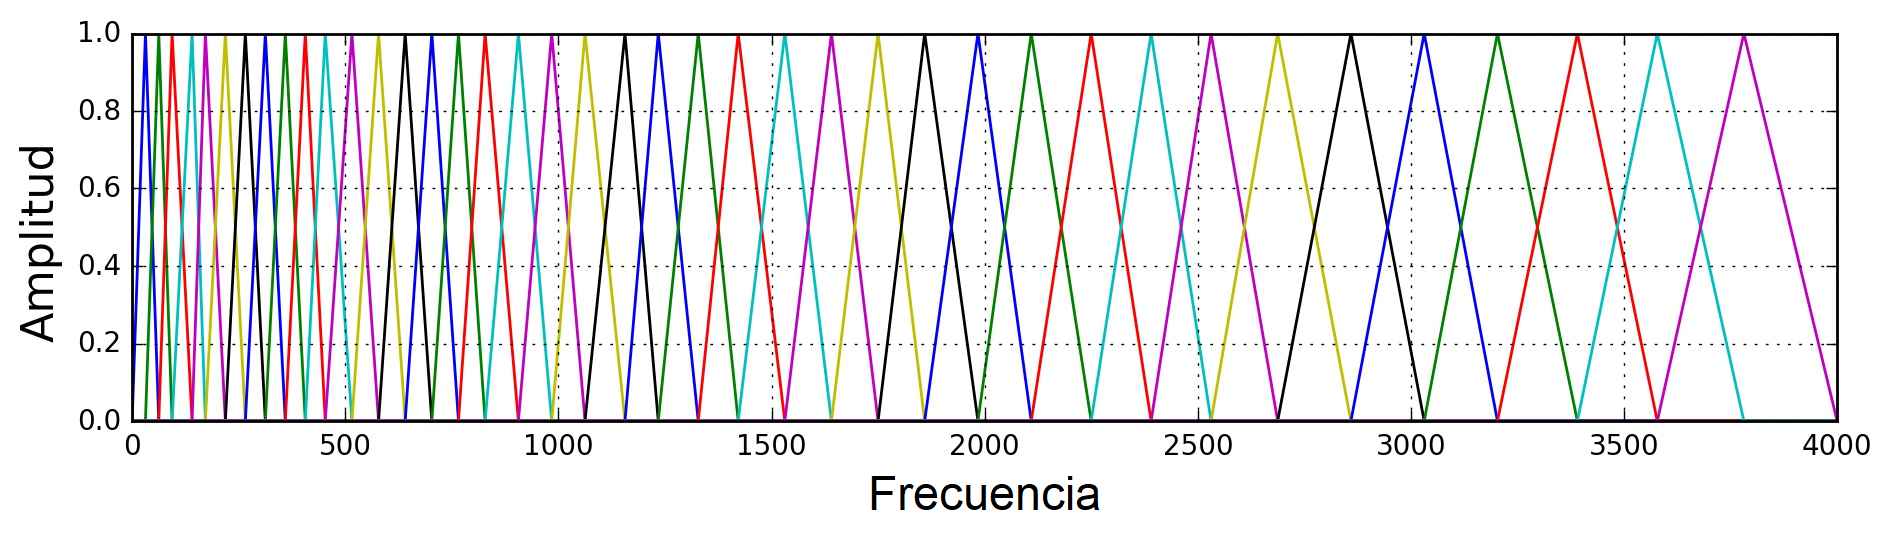
\includegraphics[width=\textwidth]{mel-filters.png}
    \caption{Banco de 40 filtros de Mel en el intervalo de frecuencias de 0~Hz a 4~000~Hz.}
    \label{img:mel-filters}
\end{figure}

A partir de todo lo anterior podemos definir el algoritmo para el cálculo de los MFCC como sigue:

\begin{algorithm}
    \caption{Cálculo de los MFCC}
    \label{algorithm:MFCC}
    Descomponer la señal $s[n]$ en tramas $s[n]_m = x[n]$ aplicando una función ventana\;
    Por cada trama calcular la potencia espectral (periodograma) a partir de su DFT, cuya $k$-ésima componente se calcula mediante la ecuación
    \[
        P[k] = \frac{|X[k]|^2}{K}
    \]
    donde $K$ es la dimensión de la DFT de la trama\;
    Aplicar el banco de filtros de Mel a $P[k]$ y sumar las energías de cada filtro.
    Aplicando $M$ filtros, se obtendrá entonces un vector de $M$ componentes (energías)\;
    Calcular el logaritmo de las energías\;
    Aplicar la transformada de coseno discreta (DCT) al vector de los logaritmos\;
\end{algorithm}

Los pasos del 1 al 4 cumplen la meta de lograr un <<resumen>> de la energía presente en la señal que se corresponda con la percepción humana del sonido.
El paso número 5, persigue eliminar la correlación entre los coeficientes.
Gracias a la aplicación de la DCT, se obtiene un vector de componentes independientes entre sí (no correlacionadas), y por lo tanto este puede ser utilizado en otros procedimientos que así lo requieran.

La DCT se calcula mediante la siguiente ecuación:
\begin{equation}
    \label{eq:DCT}
    f[j] = \sum_{m=0}^{M-1}{e[m]\cos{\left[ \frac{\pi}{M}j\left( m + \frac{1}{2} \right) \right]}}
\end{equation}

Generalmente se usan bancos de entre 20 y 40 filtros y solamente se conservan los primeros 12 o 13 coeficientes;
esto último debido a que la representación obtenida a partir de la aplicación de la DCT suele comprimir la información relevante en los primeros coeficientes, quedando poco valor en los más altos~\cite{Davis80}.

\begin{figure}[!h]
    \centering
    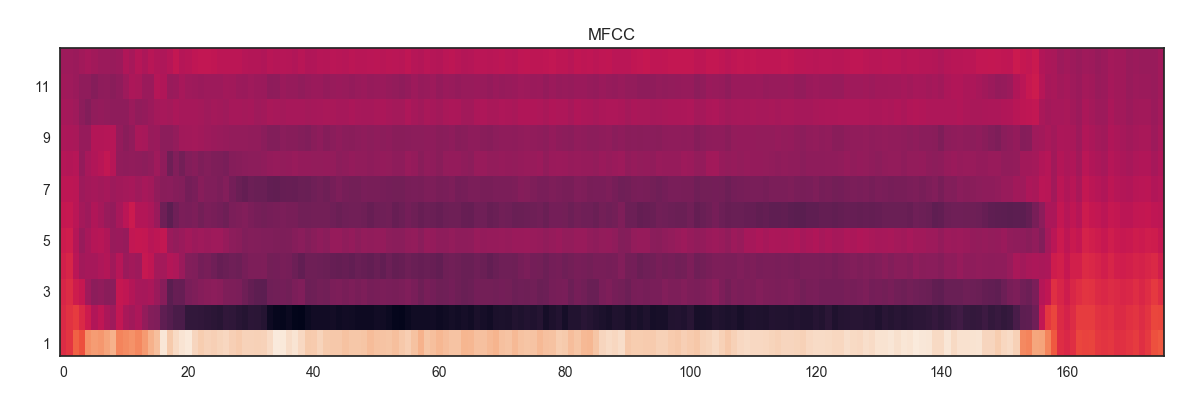
\includegraphics[width=\textwidth]{mfcc.png}
    \caption{Coeficientes MFCC del sonido de la figura~\ref{img:oscillogram}, para tramas de 1024 muestras con un tamaño de paso de 512 y empleando \textit{Hamming} como ventana.}
    \label{img:mfcc}
\end{figure}

Los coeficientes \textbf{delta} y \textbf{delta-delta}, también conocidos como \textit{diferenciales} y \textit{de aceleración} respectivamente,
constituyen una posible mejora al vector de los MFCC.
Estos incluyen información relativa al comportamiento de la energía espectral en el tiempo, que complementa la información estática de una trama que recogen los MFCC.
Para calcular los coeficientes delta aplicamos la siguiente fórmula:

\begin{equation}
    \label{eq:delta}
    d_t = \frac{\sum_{n=1}^{T}{n(c_{t+n} - c_{t-n})}}{2\sum_{n=1}^{T}{n^2}}
\end{equation}

\noindent
donde $d_t$ es el vector de coeficientes delta correspondiente a la trama $t$, y $c_{t+n}$ y $c_{t-n}$ son los MFCC de las tramas posteriores y anteriores respectivamente.
El valor de la cantidad de tramas adyacentes a explorar ($T$) suele ser 2.

Los coeficientes delta-delta pueden ser calculados de igual forma aplicando~(\ref{eq:delta}) empleando los delta en lugar de los MFCC.

A menudo sucede que un segmento de audio está compuesto por más de una trama, de manera que los procedimientos que se han descrito en esta sección producen no un único vector de características sino uno por cada trama del segmento.
Para solucionar esta situación, se construye un único vector con los promedios componente a componente de todos los de la secuencia obtenida~\cite{Lee06,Fagerlund07}.

%\section{Sumario}\label{sec:sumario}
%
%La tabla~\ref{table:features} resume las características de una señal sonora presentadas en este capítulo.
%Estas pueden agruparse por el procedimiento necesario para su cálculo en globales o por tramas;
%las primeras se computan para toda la señal, mientras que las segundas son determinadas para cada trama en que esta haya sido dividida.
%
%En el caso de ese segundo grupo, es necesario el uso de un procedimiento posterior para <<unificar>> los valores hallados para cada trama en uno que describa a la señal completa.
%Esto tiene dos finalidades: reducir la cantidad de valores que identifican a la señal según la característica en cuestión a un monto que reduzca la complejidad computacional de las operaciones sobre él;
%y producir un número fijo de valores por cada característica, lo que no es posible si se hace por tramas, dado que no todas las señales son divididas en igual cantidad de estas.
%Para la aplicación de algoritmos de inteligencia artificial sobre la señal, el segundo objetivo mencionado es especialmente importante, pues dichos algoritmos requieren que los vectores de características asociados a cada elemento del conjunto de datos posean todos la misma dimensionalidad.
%El modo en que se realiza este procedimiento varía desde la aplicación de complejas funciones específicas para la generación de nuevas características a partir de las ya calculadas~\cite{Giret11};
%hasta la simple construcción, para cada característica que así lo requiera, de un nuevo vector con las medias y las varianzas de cada componente en los vectores asociados a las tramas.
%
%\begin{table}[]
%    \centering
%    \caption{Descriptores de una señal de sonido.}
%    \label{table:features}
%    \begin{tabular}{|l|c|c|c|l}
%        \cline{1-4}
%        \multicolumn{1}{|c|}{\textbf{Característica}} & \textbf{Acrónimo} & \textbf{Por tramas} & \textbf{Dimensión} &  \\ \cline{1-4}
%        Log-Attack Time & LAT & no & 1 &  \\ \cline{1-4}
%        Audio Waveform & AWF & sí & 2 &  \\ \cline{1-4}
%        Audio Power & AP & sí & 1 &  \\ \cline{1-4}
%        Temporal Centroid & TC & no & 1 &  \\ \cline{1-4}
%        Effective Duration & ED & no & 1 &  \\ \cline{1-4}
%        Auto-Correlation & AC & sí & 1 &  \\ \cline{1-4}
%        Zero Crossing Rate & ZCR & sí/no & 1 &  \\ \cline{1-4}
%        Spectral Shape & - & sí & 3 &  \\ \cline{1-4}
%        Spectral Flux & SFX & sí & 1 &  \\ \cline{1-4}
%        Spectral Flatness & SF & sí & 1 &  \\ \cline{1-4}
%        Fundamental Frequency & F0 & sí & 1 &  \\ \cline{1-4}
%        Inharmonicity & INH & sí & 1 &  \\ \cline{1-4}
%        Odd to Even Harmonic Energy Ratio & OER & sí & 1 &  \\ \cline{1-4}
%        Tristimulus & TR & sí & 3 &  \\ \cline{1-4}
%        Mel Frequency Cepstral Coefficients & MFCC & sí & 13 &  \\ \cline{1-4}
%        \multicolumn{3}{|r|}{\textbf{Total}}                                                            & 32 &  \\ \cline{1-4}
%    \end{tabular}
%\end{table}
